%% 
%% Copyright 2007, 2008, 2009 Elsevier Ltd
%% 
%% This file is part of the 'Elsarticle Bundle'.
%% ---------------------------------------------
%% 
%% It may be distributed under the conditions of the LaTeX Project Public
%% License, either version 1.2 of this license or (at your option) any
%% later version.  The latest version of this license is in
%%    http://www.latex-project.org/lppl.txt
%% and version 1.2 or later is part of all distributions of LaTeX
%% version 1999/12/01 or later.
%% 
%% The list of all files belonging to the 'Elsarticle Bundle' is
%% given in the file `manifest.txt'.
%% 
%% Template article for Elsevier's document class `elsarticle'
%% with harvard style bibliographic references
%% SP 2008/03/01

\documentclass[preprint,12pt,authoryear]{elsarticle}

%% Use the option review to obtain double line spacing
%% \documentclass[authoryear,preprint,review,12pt]{elsarticle}

%% Use the options 1p,twocolumn; 3p; 3p,twocolumn; 5p; or 5p,twocolumn
%% for a journal layout:
%% \documentclass[final,1p,times,authoryear]{elsarticle}
%% \documentclass[final,1p,times,twocolumn,authoryear]{elsarticle}
%% \documentclass[final,3p,times,authoryear]{elsarticle}
%% \documentclass[final,3p,times,twocolumn,authoryear]{elsarticle}
%% \documentclass[final,5p,times,authoryear]{elsarticle}
%% \documentclass[final,5p,times,twocolumn,authoryear]{elsarticle}

%% For including figures, graphicx.sty has been loaded in
%% elsarticle.cls. If you prefer to use the old commands
%% please give \usepackage{epsfig}

%% The amssymb package provides various useful mathematical symbols
\usepackage{amssymb}
\usepackage{amsmath}
\usepackage{color, soul}
\usepackage{url}

\usepackage{todonotes}
\newcommand\timo[1]{\todo[inline]{Timo: #1}}

\newif\ifdetail
\detailfalse
%\detailtrue

%% The amsthm package provides extended theorem environments
%% \usepackage{amsthm}

%% The lineno packages adds line numbers. Start line numbering with
%% \begin{linenumbers}, end it with \end{linenumbers}. Or switch it on
%% for the whole article with \linenumbers.
%% \usepackage{lineno}

\journal{Physics of the Earth and Planetary Interiors}

\begin{document}

\begin{frontmatter}

%% Title, authors and addresses

%% use the tnoteref command within \title for footnotes;
%% use the tnotetext command for theassociated footnote;
%% use the fnref command within \author or \address for footnotes;
%% use the fntext command for theassociated footnote;
%% use the corref command within \author for corresponding author footnotes;
%% use the cortext command for theassociated footnote;
%% use the ead command for the email address,
%% and the form \ead[url] for the home page:
%% \title{Title\tnoteref{label1}}
%% \tnotetext[label1]{}
%% \author{Name\corref{cor1}\fnref{label2}}
%% \ead{email address}
%% \ead[url]{home page}
%% \fntext[label2]{}
%% \cortext[cor1]{}
%% \address{Address\fnref{label3}}
%% \fntext[label3]{}

\title{Free surface computations in mantle convection models}

%% use optional labels to link authors explicitly to addresses:
%% \author[label1,label2]{}
%% \address[label1]{}
%% \address[label2]{}

\author{I. Rose, B. Buffett, and Timo Heister\fnref{ref3}}

\fntext[ref3]{\url{heister@clemson.edu}, partially supported by the Computational Infrastructure in
Geodynamics initiative (CIG), through the National Science Foundation under Award No. EAR-0949446 
and The University of California-Davis, and National Science Foundation grant DMS1522191.}


\address{}

\begin{abstract}
Geodynamic simulations increasingly rely on simulations with a true free surface to 
investigate questions of dynamic topography, tectonic deformation, gravity perturbations, and
global mantle convection. However, implementations of free surface boundary conditions 
have proven challenging from a standpoint of accuracy, robustness, and stability.
In particular, free surfaces tend to suffer from sloshing instabilities, also known as 
the ``drunken sailor'' instability, which severely limit time step sizes. Several 
schemes have been proposed in the literature to deal with these instabilities.

Here we analyze the problem of creeping viscous flow with a free surface and discuss the 
origin of these instabilities. We demonstrate their cause and how existing stabilization 
schemes work to damp them out.
We also propose a new scheme for removing instabilities from free surface calculations. 
It does not require modifications to the system matrix, nor additional variables, but is instead
an explicit scheme based on nonstandard finite differences.  It relies on a single 
stabilization parameter which may be identified with the smallest relaxation timescale of the
free surface.

Finally, we discuss the implementation of a free surface in the open source, community based
mantle convection software \texttt{ASPECT}.
\end{abstract}

\begin{keyword}
%% keywords here, in the form: keyword \sep keyword

%% PACS codes here, in the form: \PACS code \sep code

%% MSC codes here, in the form: \MSC code \sep code
%% or \MSC[2008] code \sep code (2000 is the default)

\end{keyword}

\end{frontmatter}

%% \linenumbers

%% main text
\section{Introduction}
\label{sec:intro}

Surface topography in simulations of mantle convection and other geodynamic processes is an important observable,
allowing insights into Earth's internal density structure, rheology, and geoid perturbations \citep[e.g.][]{richards1984geoid, hager1985lower, baumann2014constraining}.
Historically, most simulations have been performed with free-slip boundary conditions at the surface, 
with dynamic topography calculated as a postprocessing step \citep[e.g.][]{zhong2000role}.

There have been several approaches to treating real free surfaces in geodynamic simulations.
\citet{zhong1996free} introduced a pseudo-free-surface formulation, where the free surface coordinate was
treated as an extra variable that was integrated in time. In this formulation, the free surface 
is approximated on the undeformed Eulerian grid by applying pressure boundary conditions on the reference surface.
The pressure is determined by a first-order Taylor series approximation of the hydrostatic pressure profile 
predicted by the surface topography.

A large number of studies have approximated free surfaces in the interior of the domain by using the 
`sticky air' approximation. In this approximation there is a low-viscosity, low-density layer in the fluid 
(termed `air', though its viscosity is much higher) above the free surface, effectively decoupling it from the boundary. 
Typically a free-slip boundary condition is used above the sticky air, though an open boundary may be better \citep{hillebrand2014using}. 

Finally, one can use a true free surface, where a stress-free boundary condition is applied on the boundary 
of the domain. In this case, there can be flow in and out of the domain, so the boundary must move in time.
A true free surface has mathematical elegance in that the boundary condition of the domain more closely 
matches the boundary conditions which one is trying to model, but it typically requires a deformable 
domain with frequent remeshing to avoid ill-conditioned cells. 

Recently, the nature of surface boundary conditions have been shown to be important for controlling the 
dynamics of subduction zone modeling.  In a benchmark study \citet{schmeling2008benchmark} performed extensive testing on the effect
of a free surface on the sinking of a slab. They found that the nature of the free surface had a large effect 
on the dynamics of the slab, affecting both the shape and the timing of sinking. Most of the 
participating codes in that benchmark used the sticky air approximation.
They found that the specific properties of the sticky air layer controlled the shape and timing of the slab.
Furthermore, the viscosity averaging scheme for areas of transitional
composition was extremely important, as the subducting slab entrained significant amounts of the sticky air.
\citet{crameri2012comparison} conducted comparisons between sticky air and true free surface models, 
demonstrating a range of parameters for sticky air which can mitigate some of the difficulties that it introduces.
A study by \citet{quinquis2011role} found that free surface boundary conditions have a large effect on 
trench migration in a subduction zone, and \citet{crameri2012free} found that a free surface combined 
with a weak crust is important for producing one-sided subduction zones.

All of the approaches to free surface simulations have been subject to an instability which has been 
variously termed a ``sloshing,'' or ``drunken sailor'' instability \citep{kaus2010stabilization, duretz2011discretization, kramer2012implicit}. 
This instability, arising from the large density contrast typical at a free surface (compared with the much smaller 
internal density contrasts), severely limits the maximum stable timestep for free surface computations.
Frequently, the maximum stable timestep is several orders of magnitude smaller than that for an otherwise 
equivalent model with free-slip boundary conditions.

Several studies have attempted to alleviate the timestepping requirements imposed by the sloshing 
instability. Since the most expensive part of geodynamic simulations is typically the Stokes solve,
most free surface calculations have preferred to use explicit time stepping methods for the free 
surface. \citet{kaus2010stabilization} proposed a quasi-implicit scheme which modifies the discretized 
Stokes matrix, giving it better stability properties.  \citet{kramer2012implicit} and \citet{furuichi2015implicit}
explored methods for solving the transport of the free surface implicitly.



The paper is organized as follows.
After introducing the problem in Section~\ref{sec:governing},
we derive an approach to analyze 
free surface schemes based on the normal modes in Section~\ref{sec:eigenvalue}
and Section~\ref{sec:timestepping}.
In Section~\ref{sec:kmm} we use this approach to look at the
quasi-implicit stabilization proposed in \citet{kaus2010stabilization}.
Then, we propose a new time marching scheme for free surface computations with 
good stability properties (Section~\ref{sec:newscheme}).
Finally, we describe the implementation of a free surface in the mantle convection software \texttt{ASPECT} in Section~\ref{sec:implementation}, before showing numerical results
in Section~\ref{sec:results}. 


\section{Governing Equations}
\label{sec:governing}

We begin with the incompressible momentum conservation equations for creeping incompressible flow:
\begin{equation}
\begin{aligned}
\nabla \cdot \mathbf{T} &= \rho \mathbf{g} \\
\nabla \cdot \mathbf{u} &= 0
\end{aligned}
\label{eq:momentum_mass_conservation}
\end{equation}
where $\mathbf{u}$ is the fluid velocity, $\rho$ is the fluid density, and $\mathbf{g}$ is the force due to gravity.
$\mathbf{T}$ is the stress tensor for a Newtonian fluid, defined by
\begin{equation}
\mathbf{T} = 2 \eta \varepsilon(\mathbf{u}) - p \mathbf{I}
\label{eq:stress_tensor}
\end{equation}
where $\eta$ is the viscosity and $\varepsilon(\mathbf{u}) = \frac{1}{2}(\nabla \mathbf{u} + (\nabla \mathbf{u} )^T )$ is the strain-rate tensor.
Substituting the stress tensor into Equation~\eqref{eq:momentum_mass_conservation} gets the familiar form of the Stokes equation:
\begin{equation}
\nabla \cdot \left( 2 \eta \varepsilon( \mathbf{u} ) \right) - \nabla p = \rho \mathbf{g}
\label{eq:stokes}
\end{equation}

For the purposes of this analysis it is useful to define a hydrostatic reference state where the 
velocity $\mathbf{u}$ is zero:
\begin{equation}
- \nabla p_0 = \rho_0 \mathbf{g}
\label{eq:hydrostatic_stokes}
\end{equation}
where $p_0$ is the reference hydrostatic pressure and $\rho_0$ is a reference density profile (which may vary with depth).
The total pressure and density can then be decomposed into variations about their 
reference values: $\rho = \rho_0 + \rho^\prime$, $p = p_0 + p^\prime$. 

Formally, this gives rise to the following time dependent, coupled system with unknowns $\mathbf{u}(t)$ and $\mathbf{p}(t)$:
\begin{equation}
\begin{aligned}
\nabla \cdot \left( 2 \eta \varepsilon( \mathbf{u} ) \right) - \nabla p &= \rho \mathbf{g} \qquad &\text{in} \qquad &\Omega(t)\\
\nabla \cdot \mathbf{u} &= 0  \qquad &\text{in} \qquad &\Omega(t)
\end{aligned}
\label{eq:final_system}
\end{equation}
defined on the bounded, moving domain $\Omega(t)\subset \mathbb{R}^d$ with boundary $\partial \Omega = \Gamma_0 \cup \Gamma_F$
split into a fixed (Dirichlet) and free surface part $\Gamma_0$ and $\Gamma_F$, respectively.
For the sake of economy we neglect inhomogeneous stress boundary conditions, though it would be straightforward to include them.
The domain at time $t$ is defined by advecting a reference configuration $\Omega_0$ by a mesh velocity $\mathbf{u}_{\mathrm{mesh}}(t)$
\begin{equation}
 \Omega(t) = \Omega_0 + \int_{t_0}^t \mathbf{u}_{\mathrm{mesh}}(t) \text{ d}t.
\end{equation}
The mesh velocity in normal direction is given by the velocity $\mathbf{u}(t)$ on the free surface
\begin{equation}
 \mathbf{u}_\mathrm{mesh}(t) \cdot \mathbf{n} = \mathbf{u}(t) \cdot \mathbf{n} \quad \text{on} \quad \Gamma_F
\end{equation}
and set to zero on the rest of the boundary. We defer the discussion of the velocity $\mathbf{u}_\mathrm{mesh}$ in the interior of the domain
to Section~\ref{sec:remeshing}.
Finally, we denote the displacement at time $t$ by $\zeta = \int_{t_0}^t \mathbf{u}_\mathrm{mesh}(t)\cdot \mathbf{n} \text{ d}t$, leading to the evolution
equation
\begin{equation}
\frac{\text{d} \zeta}{\text{d}t} = \mathbf{u \cdot \mathbf{n}} \quad \textrm{on  }  \Gamma_F.
\label{eq:surface_evolution}
\end{equation}



\section{Eigenvalue analysis}
\label{sec:eigenvalue}

In order to better understand the time evolution of the system in \eqref{eq:final_system}
we will consider the eigenvalues of a simplified homogeneous system. By setting $\rho = \rho_0$, we obtain the system
\begin{equation}
\begin{aligned}
\nabla \cdot \left( 2 \eta \varepsilon( \mathbf{u} ) \right) - \nabla p^\prime &= 0 \\
\nabla \cdot \mathbf{u} &= 0
\end{aligned}
\label{eq:homogeneous_stokes}
\end{equation}


We will proceed with this analysis within a finite element framework, though similar arguments should 
work for other discrete methods.
We transform the governing equations into the weak form amenable to finite elements via standard operations \citep[e.g.][]{zienkiewicz1977finite} to get

\begin{equation}
-\int_{\Omega(t)} 2 \eta \varepsilon( \mathbf{w} ) \colon \varepsilon( \mathbf{u} ) + \int_{\Omega(t)} p^\prime \nabla \cdot \mathbf{w} 
+ \int_{\Gamma_F(t)} \mathbf{w} \cdot \mathbf{T} \cdot \mathbf{n} = 0 
\label{eq:weak_stokes}
\end{equation}
\begin{equation}
\int_{\Omega(t)} q \nabla \cdot \mathbf{u} = 0
\label{eq:weak_incompressible}
\end{equation}
where $\mathbf{w}$ and $q$ are suitably chosen test functions and the integrals over 
$\Omega(t)$ and $\Gamma_F(t)$ are over the volume of the domain and the free surface, respectively.
Note that since the free surface can move, the shape of the domain is a function of time.
It is most convenient to integrate over the domain at the current timestep $\Omega^n$ 
(where the superscript indicates timestep number) instead of 
the at this point unknown $\Omega^{n+1}$. This corresponds to an explicit scheme,
which is not stable.
However, as we will see, the implicit scheme of integrating over the (unknown) domain at the correct time $\Omega^{n+1}$ will
give a stable scheme, at the cost of making the problem nonlinear \citep{furuichi2015implicit}.

The integral over the surface in Equation~\eqref{eq:weak_stokes} accounts for boundary stresses, 
which should be zero when evaluated on a true free surface.
Rather than analyzing finite deformation to the free surface (a nonlinear problem),
we will make the analytically useful approximation of small deformations about the hydrostatic 
reference surface and analyze their stability.
We will therefore  evaluate the integrals in Equation~\eqref{eq:weak_stokes} 
over the hydrostatic reference surface and introduce a temporary auxilliary variable $\zeta$ which 
represents the (small) topography of the free surface relative to that reference surface.
On the reference surface the gravity vector is opposite the direction of the surface normal $\mathbf{g} = -g \mathbf{n}$.
The stress on this reference surface can be approximated by using the first order Taylor series
expansion of the hydrostatic pressure profile:
\begin{equation}
\mathbf{T} \approx \frac{\partial \mathbf{T}}{\partial \mathbf{n} } \cdot \mathbf{n} \zeta = \rho_0 g \zeta \mathbf{I}
\label{eq:hydrostatic}
\end{equation}
Equation~\eqref{eq:weak_stokes} then becomes

\begin{equation}
-\int_{\Omega(t)} 2 \eta \varepsilon( \mathbf{w} ) \colon \varepsilon( \mathbf{u} ) + \int_{\Omega(t)} p^\prime \nabla \cdot \mathbf{w} 
+ \int_{\Gamma_F(t)} \rho_0 g \zeta  \mathbf{w} \cdot \mathbf{n} = 0 
\end{equation}

We would like to analyze the time evolution of the normal modes of this system: each mode 
is the relaxation of topography with a characteristic relaxation time.  
We denote the normal modes by $\left[ \mathbf{u}_i, p^\prime_i, \zeta_i \right]^T$, with
relaxation times $\tau_i$, where the subscript corresponds to the $i$th normal mode.

The equations decouple for the normal modes, and Equation~\eqref{eq:surface_evolution} then becomes

\begin{equation}
\frac {\text{d}}{\text{d} t} \zeta_i(\mathbf{x},t) = \frac{\text{d}}{\text{d}t} \zeta_i(\mathbf{x})e^{-t/\tau_i} = -\frac{\zeta_i(\mathbf{x},t)}{\tau_i} = \mathbf{u}_i \cdot \mathbf{n}.
\end{equation}
This can then be used to eliminate $\zeta$ from the Stokes system:
\begin{equation}
-\int_{\Omega(t)} 2 \eta \varepsilon( \mathbf{w} ) \colon \varepsilon( \mathbf{u}_i ) + \int_{\Omega(t)} p^\prime_i \nabla \cdot \mathbf{w} 
= \tau_i \int_{\Gamma_F(t)} \rho_0 g (\mathbf{u}_i \cdot \mathbf{n} ) (\mathbf{w} \cdot \mathbf{n}).
\label{eq:weak_eigen}
\end{equation}
When these equations are discretized \citep[e.g.][]{kronbichler2012high} we get
\begin{equation}
\begin{bmatrix}
A & B^T \\
B & 0 \\
\end{bmatrix}
\begin{bmatrix}
\mathbf{u}^n_i \\
p^n_i
\end{bmatrix}
=
\tau_i
\begin{bmatrix}
M & 0 \\
0 & 0
\end{bmatrix}
\begin{bmatrix}
\mathbf{u}^n_i \\
p^n_i
\end{bmatrix}
\label{eq:generalized_eigenvalue}
\end{equation}
where $\mathbf{u}^n_i$ and $p^n_i$ are finite-dimensional representations of $\mathbf{u}_i$ and $p^\prime_i$,
and $M$ is the discretization of the bilinear form on the right-hand side of Equation~\eqref{eq:weak_eigen}.

Equation~\eqref{eq:generalized_eigenvalue} is a generalized eigenvalue problem for the normal modes of the system.
It is rather more difficult to solve than a standard eigenvalue problem because the matrix on the right-hand-side 
is not invertible. It may, however, be transformed into a standard eigenvalue problem.
Define
\begin{equation}
\begin{aligned}
C &= 
\begin{bmatrix}
A & B^T \\
B & 0 \\
\end{bmatrix} \quad
D &= 
\begin{bmatrix}
M & 0 \\
0 & 0
\end{bmatrix} \quad
\mathbf{y}_i &= 
\begin{bmatrix}
\mathbf{u}^n_i \\
p^n_i
\end{bmatrix} 
\end{aligned}
\end{equation}
Then multiplying both sides by $\tau_i^{-1}C^{-1}$ we get
\begin{equation}
(C^{-1}D)\mathbf{y}_i = \tau_i^{-1} \mathbf{y}_i
\label{eq:standard_eigenvalue}
\end{equation}

This eigenvalue equation can be solved for the normal modes and relaxation times of the Stokes system with 
a free surface.

\section{Time integration of the free surface}
\label{sec:timestepping}

Armed with the normal modes and relaxation times of the Stokes system, we can write down the
formal solution to Equation~\ref{eq:surface_evolution}. Let the initial surface topography be 
represented by a linear combination of its normal modes
\begin{equation}
\zeta(\mathbf{x}, t=0) = \displaystyle \sum_i a_i \zeta_i(\mathbf{x})
\end{equation}
then the time evolution of the free surface is given by
\begin{equation}
\zeta( \mathbf{x}, t) = \displaystyle \sum_i a_i \zeta_i(\mathbf{x}) e^{-t/\tau_i}.
\end{equation}
Of course, most finite element (or finite difference, or finite volume) geodynamic simulations do not resolve 
the solution and surface topography into its normal modes and integrate those separately. 
Indeed, analytical solutions for the normal modes are only known for simple geometries and rheologies.
Instead, they obtain a velocity solution and simply advect the free surface with the local velocity.
The normal mode solution is instructive, however. 
Each mode has the form of a decay equation with characteristic decay time $\tau_i$.
The decay equation is the archetypical example of a stiff ordinary differential equation.
If we were to numerically integrate this in time with a forward Euler method, we would find the 
time-step criterion for stability \citep[e.g.][]{leveque2007finite} to be
\begin{equation}
\Delta t  \le 2 \tau_{\mathrm{min}}.
\label{eq:cfl_euler}
\end{equation}
The maximum allowable timestep is limited by the minimum relaxation timescale.
If a larger timestep than this is taken then those modes will go unstable.
The modes with the smallest relaxation times are usually those with the largest lengthscales \citep{schubert2001mantle}, 
and so it will be those which go unstable first, a phenomenon which has been called 
a ``sloshing'', or ``drunken sailor'' instability \citep{kaus2010stabilization}.

\section{Analysis of quasi-implicit stabilization}
\label{sec:kmm}

The relaxation timescales for surface topography tend to be considerably shorter than those for 
convection or tectonic deformation, so the stability requirements for a forward Euler scheme
are quite onerous.  On the other hand, an implicit time marching scheme requires solving 
a nonlinear system for the new surface position, or assembling a larger system with surface
topography unknowns \citep[e.g.][]{kramer2012implicit}.

\citet{kaus2010stabilization} proposed a scheme whereby the body forces on the domain are 
evaluated on a prediction of the shape of the domain at a later time.
The weak form of the right-hand-side body forces in the finite element discretization is then

\begin{equation}
\mathbf{f}_{\mathrm{body}} = \int_{\Omega^n + \Delta \Omega} \rho \mathbf{w} \cdot \mathbf{g}
\label{eq:predict}
\end{equation}
where the superscript $n$ on $\Omega$ indicates the shape at the $n$th timestep.
The shape prediction can be approximated by integration of the velocity:
\begin{equation}
\Delta \Omega \approx \theta \Delta t \mathbf{u}
\end{equation}
where $\theta$ is a free parameter that corresponds to the magnitude of the 
correction, where zero is no stabilization and one is fully (quasi) implicit.

One can approximately expand the integral in Equation~\eqref{eq:predict} using 
Reynold's transport theorem to find

\begin{equation}
\int_{\Omega^n + \Delta \Omega} \rho  \mathbf{w} \cdot \mathbf{g} \approx
\int_{\Omega^n} \rho  \mathbf{w} \cdot \mathbf{g} + \theta \Delta t \int_{\Gamma_F^n} \rho ( \mathbf{w \cdot g}) (\mathbf{u \cdot n} )
\label{eq:kmm}
\end{equation}
The volume integral is the same as that of the unstabilized problem, but now we obtained an additional surface integral.
It has the form of a velocity-dependent surface stress pushing down on the 
domain, and can be thought of as an artificial viscous damping of the surface.
Since the term depends on the velocity, it 
enters the system matrix as a stabilization term.  
Empirically it has been found to be successful at damping instabilities \citep{kaus2010stabilization, quinquis2011role, duretz2011discretization}.

Indeed, using the formalism in Section~\ref{sec:eigenvalue} we can see the effect of this 
stabilization term. On the reference surface we note that $\mathbf{g} = -g \mathbf{n}$, which
allows us to write the stabilization term as
\begin{equation}
-\theta \Delta t \int_{\Gamma_F^n} \rho g ( \mathbf{w \cdot n}) (\mathbf{u \cdot n} )
\end{equation}
The integral here is precisely the same as that on the right hand side of Equation~\eqref{eq:weak_eigen}, which was discretized as the matrix $M$.

If we discretize the Stokes system with the quasi-implicit stabilization term, we find
a new generalized eigenvalue problem:
\begin{equation}
\begin{bmatrix}
A + \theta \Delta t M & B^T \\
B & 0 \\
\end{bmatrix}
\begin{bmatrix}
\mathbf{u}^n_i \\
p^n_i
\end{bmatrix}
=
\tau^S_i
\begin{bmatrix}
M & 0 \\
0 & 0
\end{bmatrix}
\begin{bmatrix}
\mathbf{u}^n_i \\
p^n_i
\end{bmatrix}
\label{eq:stabilized_generalized_eigenvalue}
\end{equation}
where $\tau^S_i$ indicate the eigenvalues of the stabilized system.
This system may be rearranged:
\begin{equation}
\begin{bmatrix}
A & B^T \\
B & 0 \\
\end{bmatrix}
\begin{bmatrix}
\mathbf{u}^n_i \\
p^n_i
\end{bmatrix}
=
\left(\tau^S_i - \theta \Delta t \right)
\begin{bmatrix}
M & 0 \\
0 & 0
\end{bmatrix}
\begin{bmatrix}
\mathbf{u}^n_i \\
p^n_i
\end{bmatrix}.
\label{eq:rearranged_stabilized_generalized_eigenvalue}
\end{equation}

This is precisely the same generalized eigenvalue problem as Equation~\eqref{eq:generalized_eigenvalue},
so its eigenvalues must be the same.  This allows us to write the eigenvalues of the stabilized problem in
terms of those of the unstabilized problem:
\begin{equation}
\tau^S_i = \tau_i + \theta \Delta t
\end{equation}

Essentially, the stabilization term lengthens every relaxation time for the system by an amount $\theta \Delta t$.
This correspondingly lengthens the maximum stable timestep for the forward Euler method:
\begin{equation}
\Delta t  \le \frac{2}{1-\theta} \tau_{\mathrm{min}}.
\label{eq:cfl_euler_stabilized}
\end{equation}
Note that as $\theta$ goes to one this scheme should become unconditionally stable,
but nonlinear effects and discretization errors due to finite deformation of the surface could 
prevent that stability.

The lengthening of relaxation times due to the quasi-implicit stabilization has an unequal 
effect on the modes. They are all lengthened by the same amount, which is a much bigger 
fraction of the total relaxation time for the shorter-time modes than the longer-time ones.
Therefore the shorter-time modes are effectively damped more.
This can be seen as an attractive feature of the scheme, since those are the least stable modes,
though it can result in less accurate time-marching of the longest wavelengths of the system.

\section{A novel time-integration scheme}
\label{sec:newscheme}

One downside of the quasi-implicit scheme is that it requires a modification of the system matrix.
A naive implementation of the scheme results in a slightly 
asymmetric matrix, which can be more difficult to solve, requiring either
changes to the solver/preconditioner, or symmetrization of the stabilization term \citep{kaus2010stabilization}.
An alternative would be to construct a time-integration scheme with better stability properties.  
The reason that forward Euler integration performs so badly with the decay of topography is that 
at larger timesteps it overshoots its equilibrium position. This overshoot causes it to lurch back 
to the \emph{other} side of equilibrium, overshooting even more.
We would like to construct an explicit scheme that accounts for following properties which we know the system has:
\begin{itemize}
\item In the absence of forcing, topography always decreases.
\item Relaxation of small amplitude topography takes the form of exponential decay.
\item The decay mode with the shortest relaxation time is the least stable.
\end{itemize}

\subsection{Nonstandard finite-differences}

A general expression for the evolution of a free surface from time $t^n$ to time $t^{n+1}$ is 
\begin{equation}
\mathbf{x}(t^{n+1}) = \mathbf{x}(t^n) + \int_{t^{n}}^{t^{n+1}} \mathbf{u}(t) \text{ d}t
\label{eq:time_integration}
\end{equation}
where $\mathbf{x}$ is the location of the free surface.  If we approximate $\mathbf{u}(t) \approx \mathbf{u}(t^{n})$, 
we of course recover the forward Euler scheme.
However, we can make another choice based on our knowledge of the system behavior. 
We can approximate $\mathbf{u}(t)$ as
\begin{equation}
\mathbf{u}(t) = \mathbf{u}(t^n) e^{-(t-t^n)/\tau^*}
\label{eq:velocity_decay}
\end{equation}
where $\tau^*$ is some as-yet undetermined positive constant.
This form of $\mathbf{u}$ automatically decays in time, and as we shall see, has much better 
stability properties than forward Euler integration.
Using Equation~\eqref{eq:velocity_decay} in Equation~\eqref{eq:time_integration} and integrating, we find

\begin{equation}
\mathbf{x}(t^{n+1}) = \mathbf{x}(t^n) + \mathbf{u}(t^{n}) \tau^* \left(1-e^{-\Delta t/\tau^*} \right)
\label{eq:nsfd}
\end{equation}

The quantity $\tau^*(1-e^{-\Delta t / \tau^*})$ acts as a pseudo-timestep for advecting the free-surface.
Equation~\eqref{eq:nsfd} is what is known as a nonstandard finite-difference model, based on
constructing unusual discrete models for differential equation integration.
The theory has been developed in, among others, a series of papers by
\citet{mickens1994nonstandard, mickens2002nonstandard, mickens2005dynamic}.

\subsection{Stability of the scheme}
The parameter $\tau^*$ sets how quickly $\mathbf{u}$ decays in Equation~\eqref{eq:velocity_decay}, and a good 
choice is crucial for accuracy and stability. A shorter decay time corresponds to more stabilization,
but if it becomes too short, the surface velocity will become overdamped. In general, we will want 
to choose $\tau^*$ so that it is as close as possible to the relaxation time of the least stable mode, or $\tau_{\mathrm{min}}$.

To investigate the stability of this scheme we consider a velocity solution comprised of 
a single normal mode of the system $\mathbf{u} = a_i \mathbf{u}_i$.
This will decay exponentially with relaxation time $\tau_i$, or
\begin{equation}
\frac{\text{d} a_i} {\text{d}t} = - \frac{ a_i }{\tau_i} .
\end{equation}
Applying the nonstandard finite difference scheme, we find
\begin{equation}
a_i^{n} = a_i^{n+1} \left[ 1 - \frac{\tau^*}{\tau_i} \left(1-e^{-\Delta t/\tau^*} \right) \right].
\label{eq:recursion}
\end{equation}
In order for the scheme to be stable, the quantity in brackets must not blow up as it is repeatedly multiplied by itself, or 
\begin{equation}
\left| 1 - \frac{\tau^*}{\tau_i} \left(1-e^{-\Delta t/\tau^*} \right) \right| \le 1.
\end{equation}

\ifdetail
Taking the positive value of the absolute value yields the criterion of 
\begin{equation}
- \frac{\tau^*}{\tau_i} \left(1-e^{-\Delta t/\tau^*} \right) \le 0
\end{equation}

which can be rearranged to find
\begin{equation}
e^{-\Delta t/\tau^*} \le 1
\end{equation}

which is simply a statement that the timestep must be postive.

Taking the negative value of the absolute value yields
\begin{equation}
  \frac{\tau^*}{\tau_i} \left(1-e^{-\Delta t/\tau^*} \right)  \le 2
\end{equation}

\begin{equation}
 1 - 2 \frac{\tau_i}{\tau^*} \le e^{-\Delta t/\tau^*}
\end{equation}

if the left hand side is less than zero, then this is true regardless of step size, or
\begin{equation}
\tau^* \le 2 \tau_i
\end{equation}

if the left hand side is between zero and one, the expression is more complicated. 
Taking the log of both sides:

\begin{equation}
\Delta t \le -\tau^* \log \left(1 - 2 \frac{\tau_i}{\tau^*} \right)
\end{equation}

It is convenient to write this in terms of dimensionless times $\Delta t/ \tau_i$ and $\tau^*/\tau_i$.

\begin{equation}
\frac{\Delta t}{\tau_i} \le -\frac{\tau^*}{\tau_i} \log \left(1 - 2 \frac{\tau_i}{\tau^*} \right)
\end{equation}

\fi

The stability of this scheme is determined by the choice of $\tau^*$.  
It has a region of unconditional stability, where
\begin{equation}
\tau^* \le 2 \tau_i.
\end{equation}
Otherwise, the scheme is conditionally stable, with the timestep limited by 
\begin{equation}
\Delta t \le -\tau^* \log \left(1 - 2 \frac{\tau_i}{\tau^*} \right).
\end{equation}
The stability region is plotted in Figure \ref{fig:stability_region}. 

\begin{figure*}
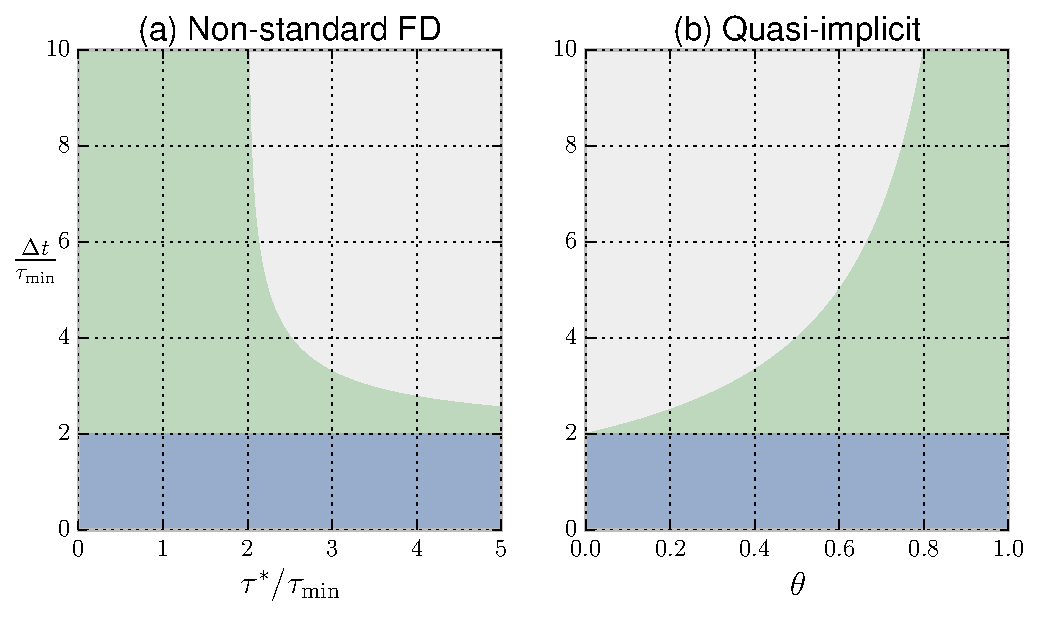
\includegraphics[width=0.9\textwidth]{figures/stability_region.pdf}
\caption{(a) Stability region for the nonstandard finite difference scheme (green). On the x-axis is the value of the stabilization time, in units of the minimum relaxation time $\tau_{\mathrm{min}}$.  On the y-axis is the value of the timestep, also in units of the minimum relaxation time. For $\tau^*\le 2 \tau_{\mathrm{min}}$ the nonstandard finite difference scheme is unconditionally stable.  (b) Stability region for the quasi-implicit scheme (green).  Again, the y axis is in units of the minumum relaxation time.  The x-axis shows the value of the stabilization parameter $\theta$. For $\theta = 1$ the quasi-implicit scheme is unconditionally stable. In both cases the stability region for the forward Euler scheme is also shown in blue.}
\label{fig:stability_region}
\end{figure*}

\subsection{Accuracy and asymptotics of the scheme}
It is important to note that even though we derived the nonstandard finite difference scheme assuming a decaying exponential
for $\mathbf{u}$, it is formally a first-order accurate scheme. As such, it is capable of capturing arbitrary motions 
of the free surface, but with better stability properties than forward Euler schemes.

Again we may take one of the normal modes as an example and inspect the difference between the nonstandard finite-difference
scheme and the analytical solution after one time step:

\begin{equation}
\begin{aligned}
a_i(\Delta t) - a_i^{1} &= a_i(0) e^{-\Delta t/\tau_i} - a_i{(0)} \left[ 1 - \frac{\tau^*}{\tau_i} \left(1-e^{-\Delta t/\tau^*} \right) \right] \\
                        &= a_i{(0)} \left[ e^{-\Delta t/\tau_i} - 1 + \frac{\tau^*}{\tau_i} \left(1-e^{-\Delta t/\tau^*} \right) \right].
\end{aligned}
\end{equation}
Note that when $\tau_i = \tau^*$ the nonstandard finite difference scheme is exact.
The exponentials may be expanded to find
\ifdetail
\begin{equation}
a_i(\Delta t) - a_i^{1} = - a_i{(0)} \left[ \left(\frac{\Delta t}{\tau_i}\right)^2 - \frac{\tau^*}{\tau_i} \left(\frac{\Delta t }{\tau^* }\right)^2 \right].
\end{equation}
\fi
\begin{equation}
a_i(\Delta t) - a_i^{1} = {a_i{(0)} } \left( \frac{\Delta t}{\tau_i} \right)^2 \left( 1 - \frac{\tau_i}{\tau^*} \right) + O(\Delta t^3).
\end{equation}
Summing this error over many timesteps results in a factor of $\Delta t^{-1}$, demonstrating the first-order accuracy~\citep[e.g.]{leveque2007finite}.
The choice of $\tau^*$ controls the size of the coefficient on the truncation error for the scheme.
The error for a given mode becomes considerably smaller when $\tau^*$ is close to its natural relaxation times.

It is helpful to take a closer look at the pseudo-timestep introduced in Equation~\eqref{eq:nsfd}: $\tau^*(1-e^{-\Delta t/\tau^*})$.
As the timestep $\Delta t$ goes to zero, the pseudo timestep approaches $\Delta t$, recovering 
the forward Euler scheme. However, as $\Delta t$ gets larger, the pseudo-timestep does not 
increase as quickly, reflecting the decaying nature of the normal modes.
Likewise, as the stabilization timescale $\tau^*$ goes to infinity, we also recover the 
forward Euler scheme, in what is essentially the unstabilized problem. But as $\tau^*$
goes to zero, the pseudo-timestep also goes to zero. This corresponds to over-stabilizing the
problem. With too short of a stabilization timescale the free surface is never advected 
at all (which is a very stable situation, if not very accurate!).

\subsection{Choice of $\tau^*$}
As discussed above, a full geodynamic simulation will have a spectrum of relaxation times.
For complete stability, the parameter $\tau^*$ should be chosen such that every mode is stable.
In practice, this means that a good choice is 
\begin{equation}
\tau^* \approx \tau_{\mathrm{min}}.
\label{eq:tau_choice}
\end{equation}

Unfortunately, for many models the minimum relaxation time will not be known beforehand. 
In order to use the nonstandard finite difference scheme, the value of $\tau^*$ would need 
to be calculated or estimated first.  There are several possible ways to determine this value:

\begin{itemize}
\item Direct solution of Equation~\eqref{eq:generalized_eigenvalue}. This can be expensive, although
only the minimun relaxation time is required. For certain geometries a simple power iteration on 
the standard eigenvalue problem~\eqref{eq:standard_eigenvalue} could be enough.
\item Analytical formulae. Several geometry and viscosity model combinations have analytical solutions
for relaxation spectra. Even if the user's model is not precisely the same (e.g., has some lateral viscosty
variations), an analytical approximation may be sufficient.
\item Scaling. In general, we expect the relaxation times to scale with $\tau \sim \frac{\eta}{\rho g L}$,
where the density, gravity, viscosity, and lengthscale are all representative values.  A small amount
of experimentation near this value of $\tau$ can find an appropriate relaxation time.
\item Observation of instabilities.  The mere act of observing a sloshing instability in an unstabilized
problem can furnish an estimate of its relaxation time.
\end{itemize} 


\section{Implementation in \texttt{ASPECT} }
\label{sec:implementation}
We have implemented the ability to run free surface simulations in the mantle convection software \texttt{ASPECT} \citep{kronbichler2012high}. 
\texttt{ASPECT} is designed to be highly flexible and modular, with the ability for user-defined rheologies, geometries, and gravity models. 
The implementation of the free surface, therefore, needs to be general enough to work for many combinations of these models, including those 
which may not have been written yet. In particular, it cannot rely on assumptions regarding the shape of the domain.

Furthermore, \texttt{ASPECT} allows for computations in both 2D and 3D, so the implementation must be sufficiently dimension
independent to work in both cases. We implement the free surface within an arbitrary Lagrangian-Eulerian (ALE) formulation
\citep[e.g][]{fullsack1995arbitrary,donea2004encyclopedia}.

\texttt{ASPECT} is a parallelized, distributed memory code with adaptive mesh refinement.
The free surface implementation works with these features.  We store the mesh vertex positions 
in a fully distributed vector. This vector is continually updated and redistributed across 
processes upon mesh adaptation (which is handled by the adaptive octree library \texttt{p4est}).
We also provide adaptive refinement indicators based on being near to the free surface or 
when the free surface slope is steep to allow for accurate interface tracking.


\subsection{Remeshing}
\label{sec:remeshing}

In ALE calculations the internal mesh velocity is undetermined.
In general, one wants to smoothly deform the mesh so as to preserve its regularity, 
avoiding inverted or otherwise poorly conditioned cells.
The mesh deformation can be calcluated in many different ways, including algebraic \citep[e.g.][]{thieulot2011fantom} 
and PDE based approaches.

We choose to implement remeshing based on solving Laplace's equation for the mesh velocity.
We solve the equation
\begin{equation}
\nabla^2 \mathbf{u}_{\mathrm{mesh}} = 0
\label{eq:laplacian_smoothing}
\end{equation}
subject to the boundary conditions
\begin{equation}
\begin{aligned}
&\mathbf{u}_\mathrm{mesh} = 0 & \qquad & \textrm{on } \Gamma_0. \\
&\mathbf{u}_\mathrm{mesh} = \left( \textbf{u} \cdot \textbf{n} \right) \textbf{n} & \qquad & \textrm{on } \Gamma_F, \\
&\mathbf{u}_\mathrm{mesh} \cdot \textbf{n} = 0 & \qquad & \textrm{on } \Gamma_{FS}, \\
\end{aligned}
\label{eq:laplacian_bcs}
\end{equation}
where $\Gamma_{FS}$ is the part of the boundary with free slip boundary conditions $\mathbf{u \cdot n} = 0$.
This scheme has the advantage of working for many different domain geometries and combinations of boundary conditions.
For moderate mesh deformation, the mesh stays smooth and well conditioned, though it breaks down for large deformations 
or on non-convex domains.

\subsection{Surface advection}
With a deformable domain there is the danger that small errors in free surface motion can
result in poor overall mass conservation in time. In some scenarios, the total volume of the mesh can 
fluctuate significantly over hundreds or thousands of time steps.
Consistency with the Stokes solution requires 
\begin{equation}
\mathbf{u}_{\mathrm{mesh}} \cdot \mathbf{n} = \mathbf{u \cdot n}.
\end{equation}

Unfortunately the normal vectors are not well defined on the mesh vertices, which is 
where the mesh velocity is defined. One could instead advect the mesh in the direction 
of the local vertical, or in some weighted average of the cell normals adjacent to a given vertex,
but we have found that these schemes do not necessarily have good mass conservation 
properties.

A better approach is to perform a finite element projection of the Stokes velocity 
solution onto the mesh velocity vector. Multiplying the boundary conditions 
\eqref{eq:laplacian_bcs} by a test function $\mathbf{w}$ and integrating over the free
surface part of the boundary, we find

\begin{equation}
\int_{\Gamma_F} \mathbf{w} \cdot \mathbf{u}_\mathrm{mesh} = 
\int_{\Gamma_F} \left( \mathbf{w \cdot n } \right) \left( \mathbf{u \cdot n} \right).
\end{equation}
When discretized, this forms a linear system which can be solved for the mesh velocity $\mathbf{u}_\mathrm{mesh}$ at the 
free surface. Of course, a new system to solve is not ideal, but this system, being nonzero 
over only the free surface, is relatively small and easy to solve.

This weak solution to the boundary conditions~\eqref{eq:laplacian_bcs} is able to borrow
the accuracy of the Stokes solve for Equation~\eqref{eq:weak_incompressible}, and we have 
found it to conserve mass more accurately than algebraic techniques for evaluating the mesh-normal velocity.
Similar results were found by \citet{fullsack1995arbitrary}.

\section{Numerical Results}
\label{sec:results}

We demonstrate the convergence of the nonstandard finite difference model by comparison 
with an analytical solution. Following \citet{kramer2012implicit} we model the relaxation
of sinusoidal surface topography in a two-dimensional Cartesian box with an isoviscous fluid.
The setup is shown in Figure~\ref{fig:benchmark_setup}.

The initial topography is given by
\begin{equation}
\zeta(x,0) = \zeta_0 \cos\left( k x \right)
\end{equation}
where $k = 2 \pi / L$.

The time evolution of this topography is then
\begin{equation}
\zeta(x, t) = \zeta(x,0) e^{-t/\tau}
\end{equation}
where the relaxation time $\tau$ is given by
\begin{equation}
\tau = \frac{D k + \sinh(D k) \cosh(D k)}{ \sinh^2 (D k) } \frac{2 k \eta}{\rho g}
\end{equation}
where $D$ is the layer depth, $\eta$ is the viscosity, $\rho$ is the density, and $g$ is the force of gravity.

This solution is only valid for infinitesimal topography. However, for small
initial topography $\zeta_0$ it seems to be sufficiently accurate to test convergence orders up 
to quadratic \citep{kramer2012implicit, furuichi2015implicit}.
We evaluate error by time-integrating the L2 difference between the numerical and analytical
solutions at the center of the domain:
\begin{equation}
\mathrm{Error} = \frac{1}{4\tau}\int_0^{4 \tau} \lVert \zeta_\mathrm{numeric}(L/2, t) - \zeta_\mathrm{analytic}(L/2, t) \rVert_2 \text{ d}t.
\end{equation}

\begin{figure*}
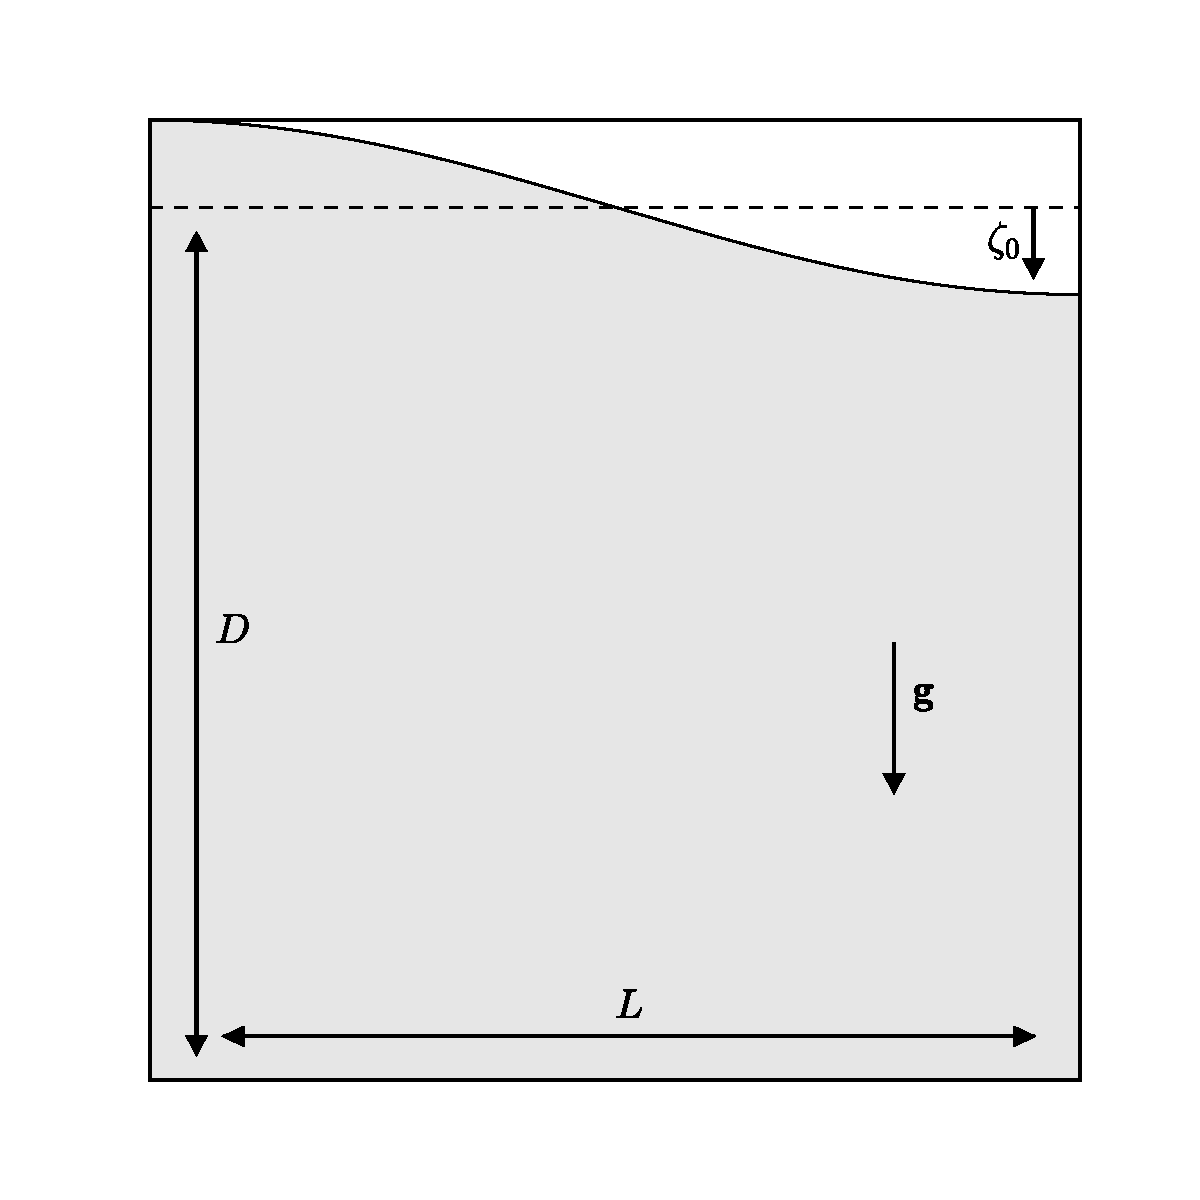
\includegraphics[width=0.9\textwidth]{figures/benchmark_setup.pdf}
\caption{Setup for the free surface relaxation benchmark. A 2D box with an isoviscous fluid has sinusoidal initial topography, with amplitude $\zeta_0$. The box has depth $D$ and length $L$. For our tests $\rho = \eta = g = D = L = 1$, and $\zeta_0 = 0.005$.}
\label{fig:benchmark_setup}
\end{figure*}

Figure~\ref{fig:timestep_convergence}a shows the convergence of the nonstandard finite difference scheme 
with respect to timestep size. The scheme is first order in time, with improving accuracy as the value of $\tau^*$ approaches
the relaxation time of the relevant mode $\tau_i$. Interestingly, if $\tau^* = \tau_i$ the advection scheme
becomes exact \citep{mickens2002nonstandard}. At this point the magnitude of the error plummets and is no longer 
a strong function of the timestep. The remaining error is likely due to error in the linear approxmation for 
the analytical solution, the spatial discretization, or the linear solver tolerance. 

Figure~\ref{fig:timestep_convergence}b shows the convergence of the quasi-implicit scheme with timestep.
When $\theta=0$, it corresponds to the unstabilized forward Euler scheme, and is first order in time. 
When $\theta=1$ it is also first order in time, but allows for a much larger timestep.  When $\theta=0.5$
the quasi-implicit guess for the body force is good enough that it actually seems to achieve the second-order 
convergence of a trapezoidal scheme, though it is not clear whether this extends to more complicated models.

Figure~\ref{fig:tau_sensitivity} shows in more detail the effects of the choice of $\tau^*$. In a narrow region 
close to the true value of $\tau_\mathrm{min}$ the error becomes very small, but in a broader region nearby 
the errors are larger. 
The excellent accuracy when the stabilization timescale $\tau^*$ is close to one of the natural relaxation
timescales allows for tuning of the scheme to track specific long-wavelength modes, such as 
those due to rotational or tidal deformation.

\begin{figure*}
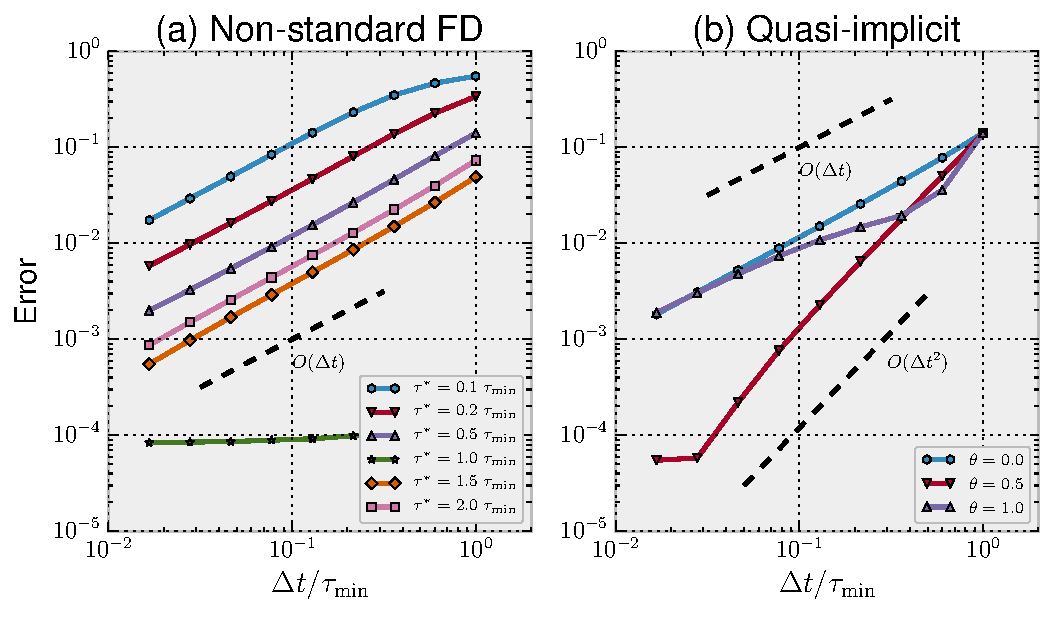
\includegraphics[width=0.95\textwidth]{figures/timestep_convergence.pdf}
\caption{Convergence tests for the benchmark shown in Figure~\ref{fig:benchmark_setup}. (a) Convergence test with timestep size for the nonstandard finite difference scheme. Comparison with the slope-one line confirms that it is first-order in time. In the case that the stabilization relaxation time $\tau^*$ is equal to the analytic relaxation time the error becomes very small, as the time integration scheme becomes exact \citep{mickens2002nonstandard}. (b) Convergence test with timestep size for the quasi-implicit scheme. For $\theta = 1$ and $\theta = 0$ the scheme is first-order accurate (though the latter is just an unstabilized forward-Euler scheme). For $\theta=0.5$ the scheme appears second order accurate on this benchmark.}
\label{fig:timestep_convergence}
\end{figure*}

\begin{figure*}
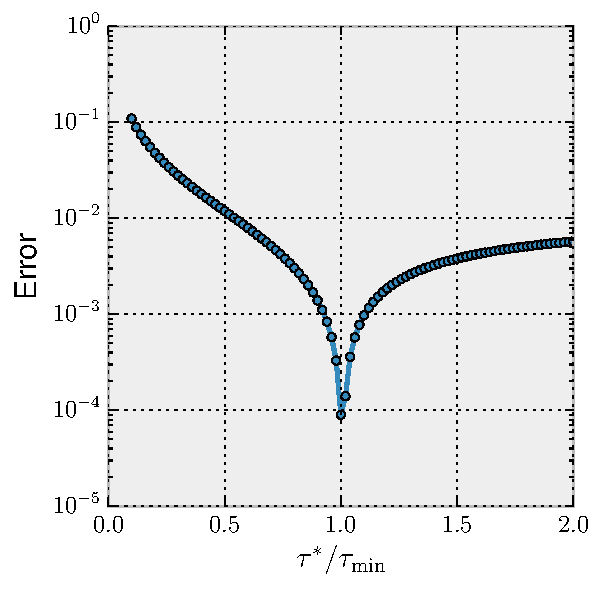
\includegraphics[width=0.9\textwidth]{figures/tau_sensitivity.pdf}
\caption{Sensitivity of the nonstandard finite difference scheme to $\tau^*$. As the relaxation parameter $\tau^*$ approaches the relaxation time of the benchmark case the error reduces. The sharp cusp at $\tau^* = \tau_\mathrm{min}$ corresponds to the almost spectral accuracy of the time marching scheme for that case.}
\label{fig:tau_sensitivity}
\end{figure*}

We also investigate the advantages of combining adaptive mesh refinement with free surface computations.
\citet{crameri2012comparison} performed a community benchmark of a setup for which there is no analytic
solution. In this benchmark, a buoyant blob rises beneath a viscous lid with a free surface, deflecting the
boundary upwards (for the full setup, see \citet{crameri2012comparison}). 
Figure~\ref{fig:amr} shows the convergence of the maximum topography at 3 Myr to its value in a high resolution simulation,
both with and without adaptive mesh refinement.
For the uniform refinement cases each point is generated by running the benchmark with a different global refinement level.
For the adaptive case each point is generated by allowing the mesh to be refined, where the maximum refinement level
is limited to the same refinement level of the corresponding global refinement simulation.
We refine every ten timesteps according to gradients in the density and compositional fields.

The convergence with and without adaptive mesh refinement have essentially the same behavior, but the adaptive case requires 
fewer degrees of freedom by a factor of approximately an order of magnitude. More complex models will have
more detail and so we may be less able to aggressively coarsen them, but we still expect that adaptive mesh refinement 
will result in significant computational savings.

\begin{figure*}
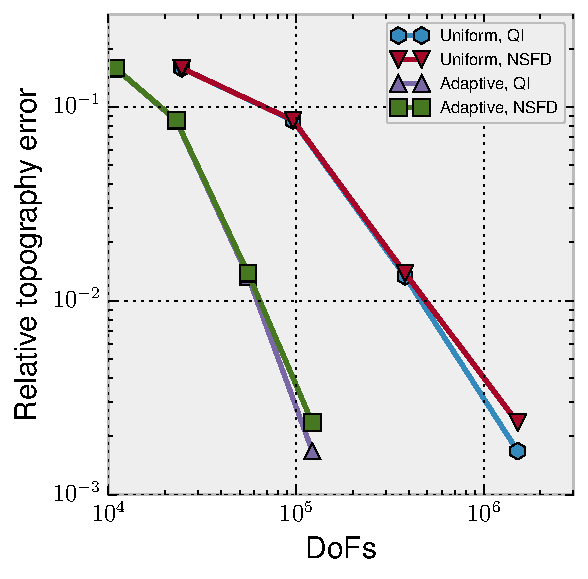
\includegraphics[width=0.9\textwidth]{figures/amr.pdf}
\caption{Convergence with degrees of freedom (DoFs) for the \citet{crameri2012comparison} Case 2 benchmark, for both uniform and adaptive mesh refinement. The timestep $\Delta t$ is 500 yr. We compare the maximum topography at 3 Myr with its value at high resolution ($\sim$398 m). For the adaptive cases we perform mesh refinement according to the sum of density and composition gradients. Both cases converge similarly, but the adaptive mesh refinement simulations require significantly smaller system sizes.}
\label{fig:amr}
\end{figure*}

\section{Conclusion}
We have analyzed stability of free surface boundary conditions in geodynamic simulations and 
demonstrated the cause of sloshing instabilities using a normal mode analysis.
This perspective on the problem allowed us to construct an explicit finite difference 
scheme which is first order accurate in time and is unconditionally stable.
The nonstandard finite difference scheme is extremely simple to implement, and 
requires no modifications to the system matrix.

The normal mode perspective on the problem also provides insights into the effect of 
the quasi-implicit stabilization scheme proposed by \citet{kaus2010stabilization}.
The relaxation time of each mode is lengthened by an amount $\theta \Delta t$, and the
maximum allowable timestep is correspondingly lengthened.

It is not clear that the non-standard finite difference scheme is superior to 
the quasi-implicit scheme. For $\theta=0.5$ the quasi-implicit scheme is more accurate,
but is only conditionally stable. For $\theta=1$ the two schemes are comparably accurate 
in the tests we ran.

Finally, we have described the implementation of free surface boundary conditions in 
the open source mantle convection software \texttt{ASPECT}. Both the quasi-implicit 
scheme and the nonstandard finite difference scheme are available. The implementation is 
sufficiently general to accommodate many different geometies, rheologies, and 
gravity models. Furthermore, it runs in parallel and with adaptive mesh refinement.

%% The Appendices part is started with the command \appendix;
%% appendix sections are then done as normal sections
%% \appendix

%% \section{}
%% \label{}

%% If you have bibdatabase file and want bibtex to generate the
%% bibitems, please use
%%
\section{Bibliography}
\bibliographystyle{elsarticle-harv} 
\bibliography{free-surface-paper}

%% else use the following coding to input the bibitems directly in the
%% TeX file.

%\begin{thebibliography}{00}

%% \bibitem[Author(year)]{label}
%% Text of bibliographic item

%\bibitem[ ()]{}

%\end{thebibliography}
\end{document}

\endinput
%%
%% End of file `elsarticle-template-harv.tex'.
